% !TEX program = xelatex
\documentclass[
  10pt,
  twoside,
  openany,
  b5paper, % 以上均为 ctexbook 提供的文类选项
  colorscheme = basic, % 请根据需要选择或定制配色方案
]{qyxf-book}

\usepackage[contents = 钱院学辅, scale = 15, color = black, angle = 50, opacity = .10]{background}
\usepackage{pdfpages}
\includepdfset{pagecommand={\thispagestyle{plain}}}

\title{电路课件与笔记}
\subtitle{Slides and Notes of Circuit}  % 可选
\author{邹建龙\ 电气钱82班蔡易骎}
\date{2020 年 1 月 6 日}
\typo{张露承\ 宋仁静}

% 定制元信息
\org{\Large\textit{钱学森书院学业辅导中心}\\\textsc{Qian Xuesen College Academic Counseling Center}}
\footorg{\textsc{Qian Yuan Xue Fu}}
\cover{
	\begin{tikzpicture}[remember picture, overlay]
		\begin{pgfonlayer}{background}
			\node at ($(current page.east)+(0in,0in)$){
				
\includegraphics[width=.8\textwidth]{cover.png} };
		\end{pgfonlayer}
	\end{tikzpicture}
}
\license{}  % 清空许可证信息

% 调整封面标题大小
\renewcommand{\titlefont}{\Huge\bfseries}
\renewcommand{\subtitlefont}{\LARGE\itshape}

\begin{document}

\maketitle

\chapter*{前言}
\thispagestyle{empty}

电路是一门很基础也很重要的课程,如果掌握得扎实,对后面信号与系统,模电和数电等课程学习有很大的帮助,使用起来也会得心应手。

我自己将电路的学习分为三个方面,一是电路的基本概念,二是电路分析的基本定理和定律,三是电路学习的一些思维方式。

电路的基本概念虽然看起来不难,但要很熟悉却属实不易。例如三相电路的各种功率,我们需要知道的绝不仅仅是它们的符号和计算公式,更应该清楚它们是怎么定义的,为什么要这样定义,在实际中什么时候需要用到哪种功率,概念掌握更上一层后还应清楚它们之间的相互关系。很多概念的意思从它们的名字其实就可以知道个大概,适当联想可以清楚地记得,可以避免硬背。

电路分析的基本定律和定理往简单了说有三个,KVL,KCL,VCR,由此可以得到几乎所有电路的分析方法,比如由此而来的结点电压法和回路电流法,比如分压分流定律,再到分析系统的微分方程和传递函数,都是根据KVL,KCL和电阻、电感和电容的VCR得来的。知道这些后,对题目的分析和求解可以保持清醒和“俯视”,不至于被绕进去。

最后是一些巧妙的思想方法,也是我以为电路学习最重要的东西,比如学习的特勒根定理,去耦等效,戴维宁等效等,都是为了简化电路,便于清楚分析的重要工具。在学习的可以带着“为什么要这样变换”“这样变换为什么可行”“变换前后有什么区别”“变换的具体适用条件是什么”等问题,思考一下,或许会有意想不到的收获。

知识的具体内容我们可能学完就忘,但巧妙的思考方式是受用不尽的财富。

\rightline{——电气钱82班\ 蔡易骎} 

\newpage
\tableofcontents

\newpage
\addcontentsline{toc}{chapter}{2 KCL、KVL}
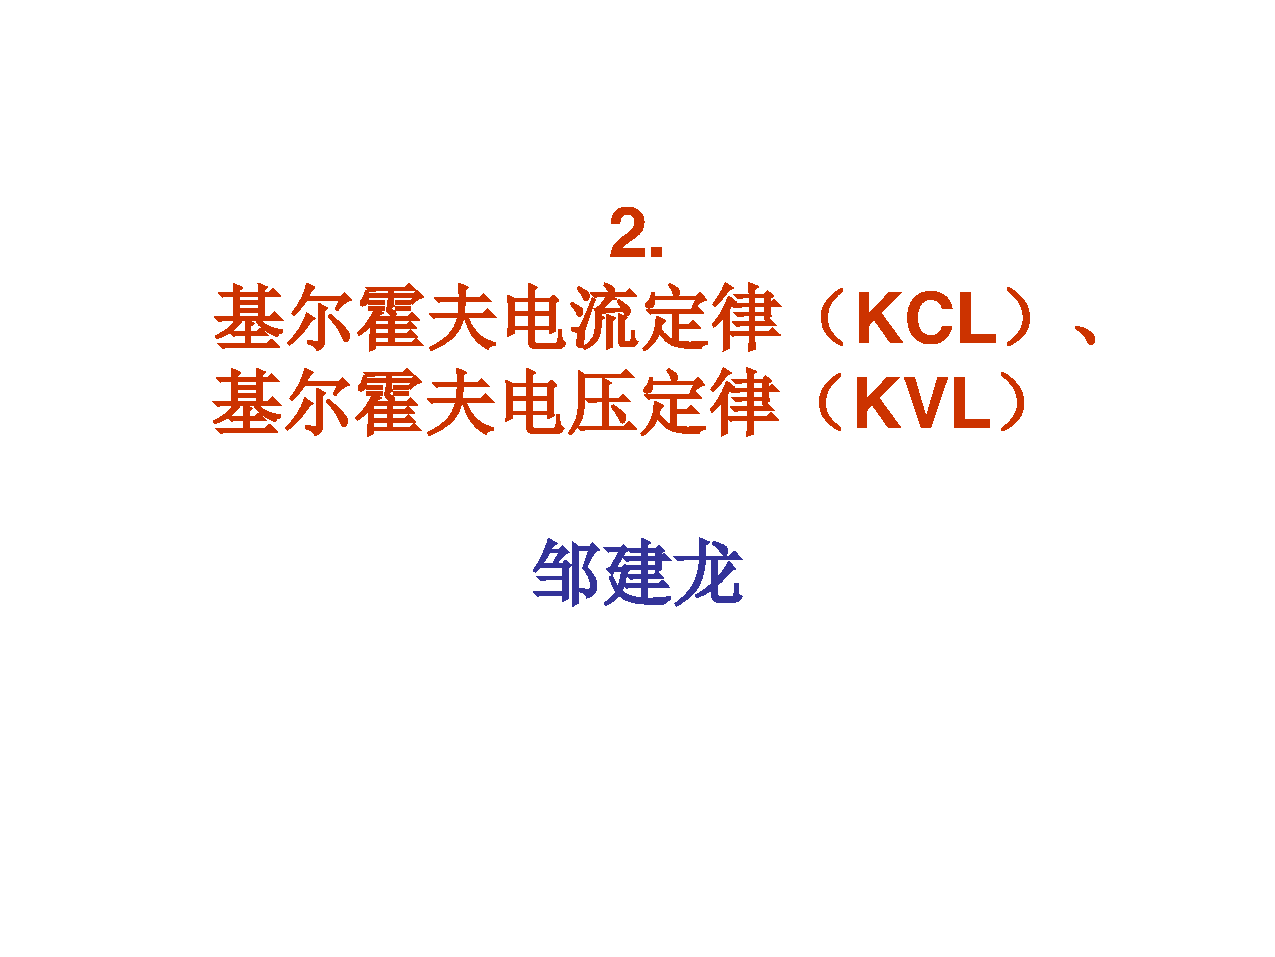
\includepdf[pages = - , nup=2x3]{content/Circuit(1).pdf}
\addcontentsline{toc}{chapter}{3 电路的等效变换}
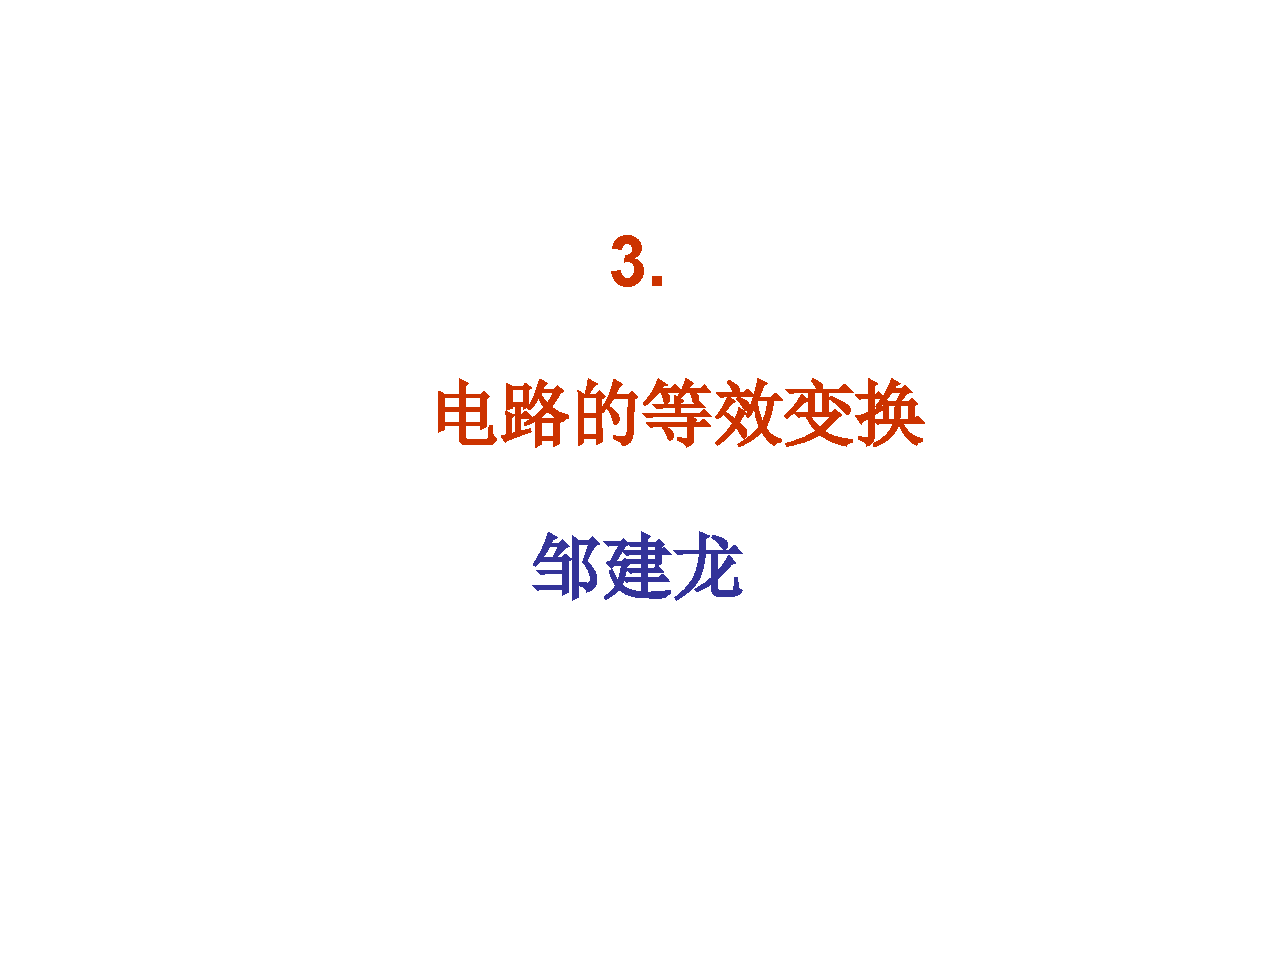
\includepdf[pages = - , nup=2x3]{content/Circuit(2).pdf}
\addcontentsline{toc}{chapter}{4 电路的图}
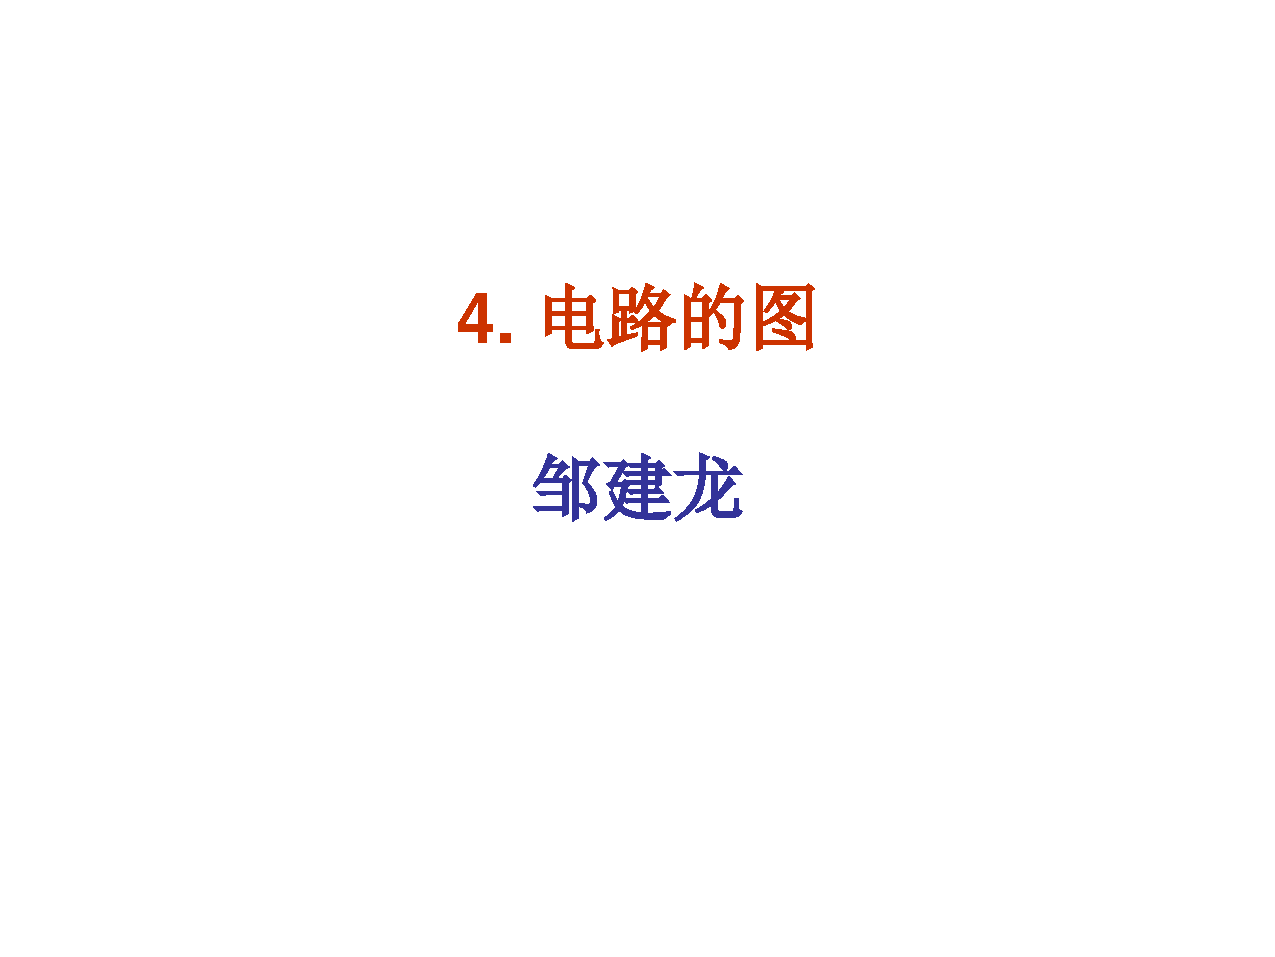
\includepdf[pages = - , nup=2x3]{content/Circuit(3).pdf}
\addcontentsline{toc}{chapter}{5 回路电流法}
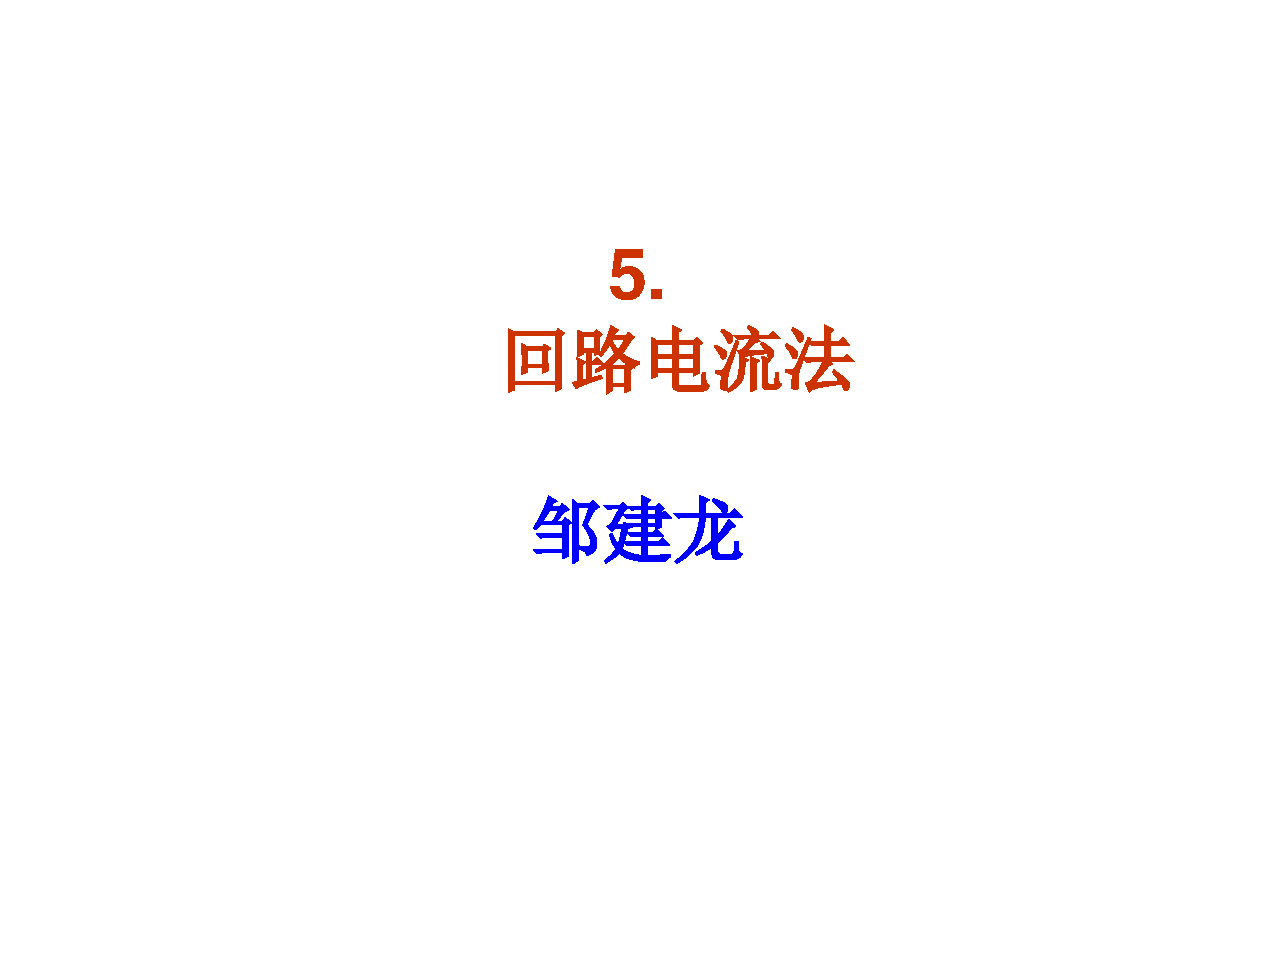
\includepdf[pages = - , nup=2x3]{content/Circuit(4).pdf}
\addcontentsline{toc}{chapter}{6 结点电压法}
\includepdf[pages = - , nup=2x3]{content/Circuit(5).pdf}
\addcontentsline{toc}{chapter}{7 叠加定理、齐性定理和替代定理}
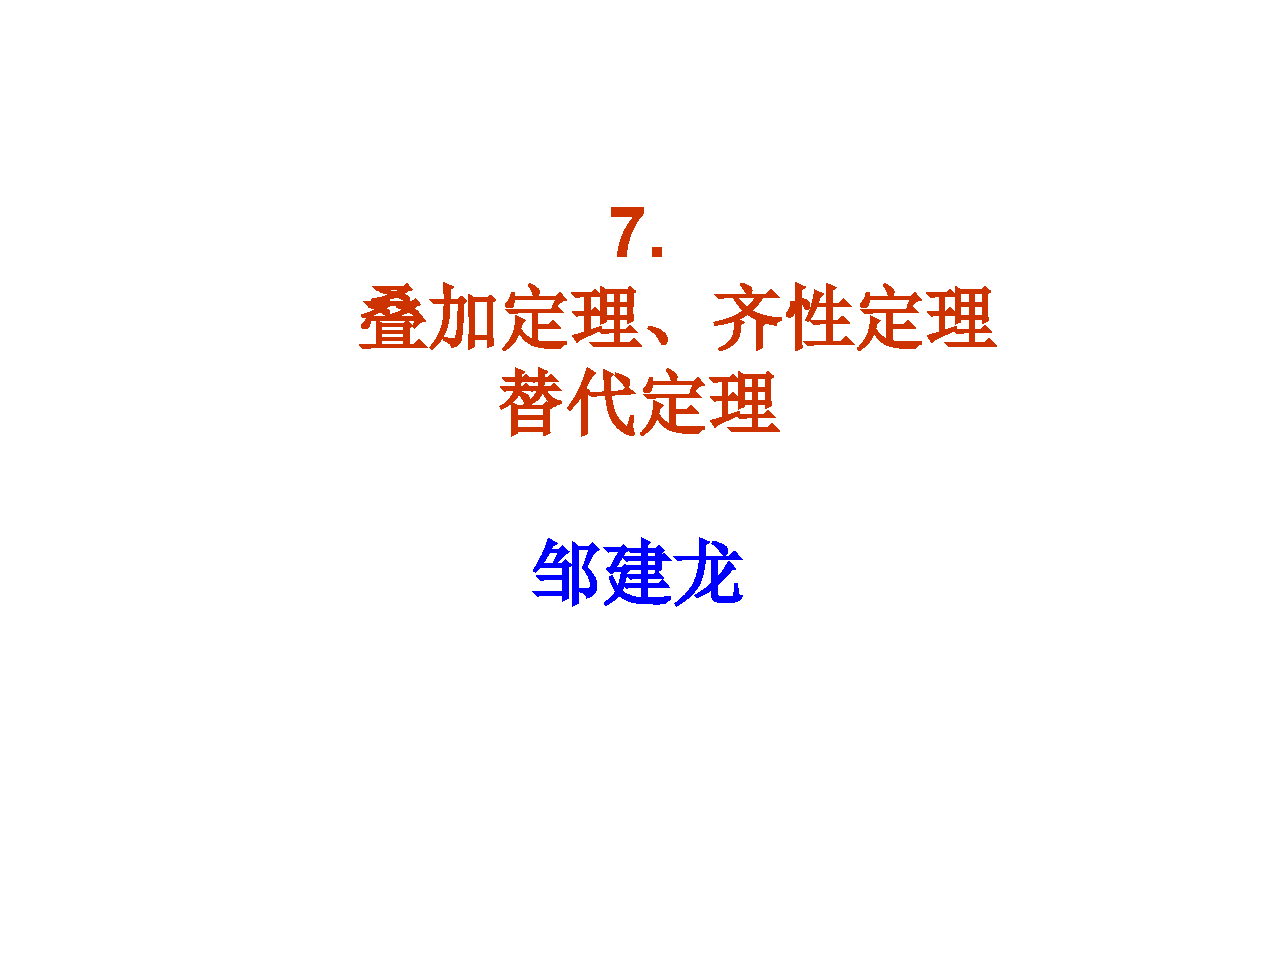
\includepdf[pages = - , nup=2x3]{content/Circuit(6).pdf}
\addcontentsline{toc}{chapter}{8 戴维宁定理和诺顿定理}
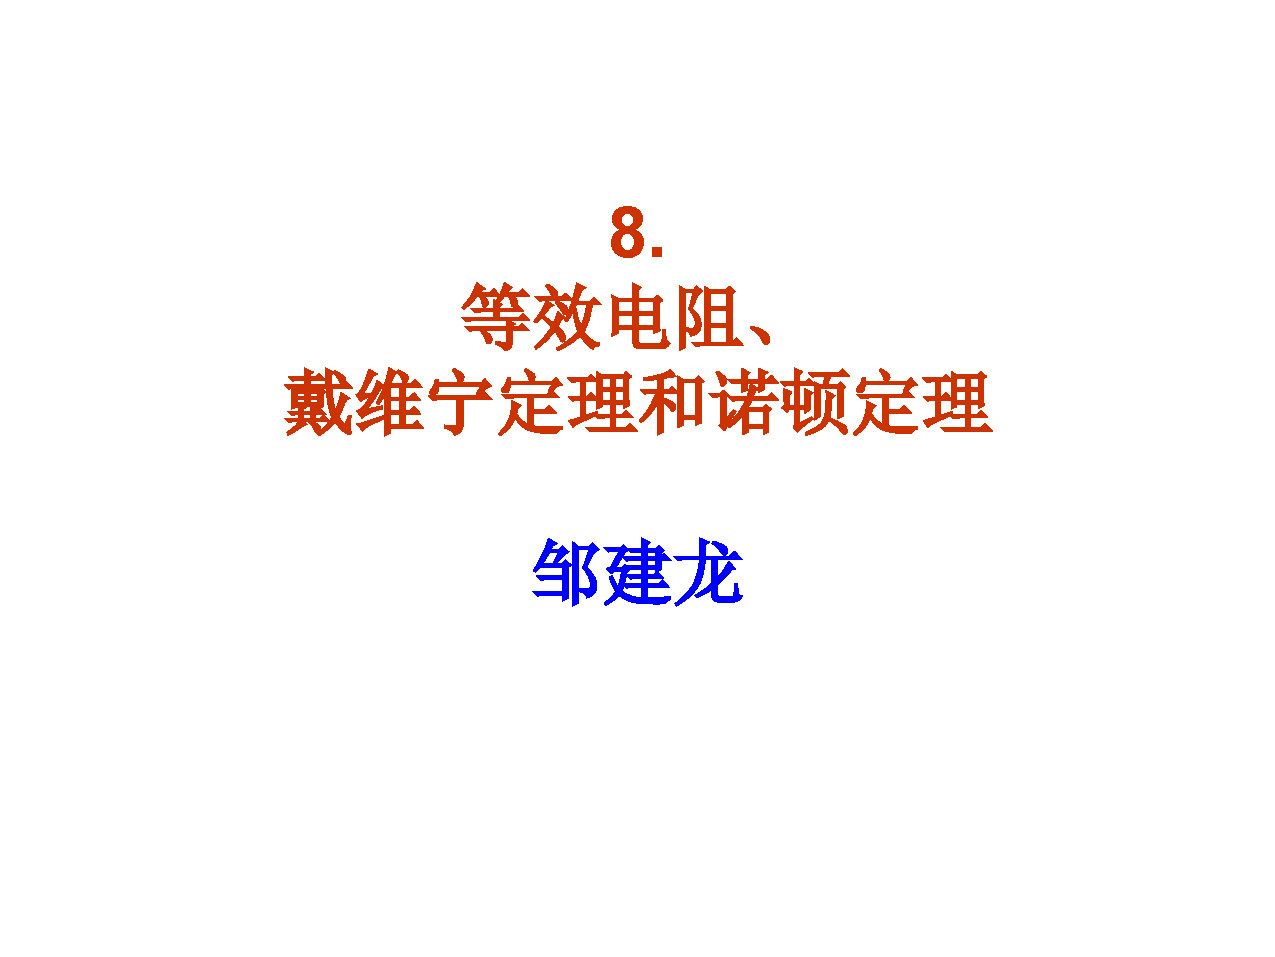
\includepdf[pages = - , nup=2x3]{content/Circuit(7).pdf}
\addcontentsline{toc}{chapter}{9 戴维宁等效电路求解及其应用}
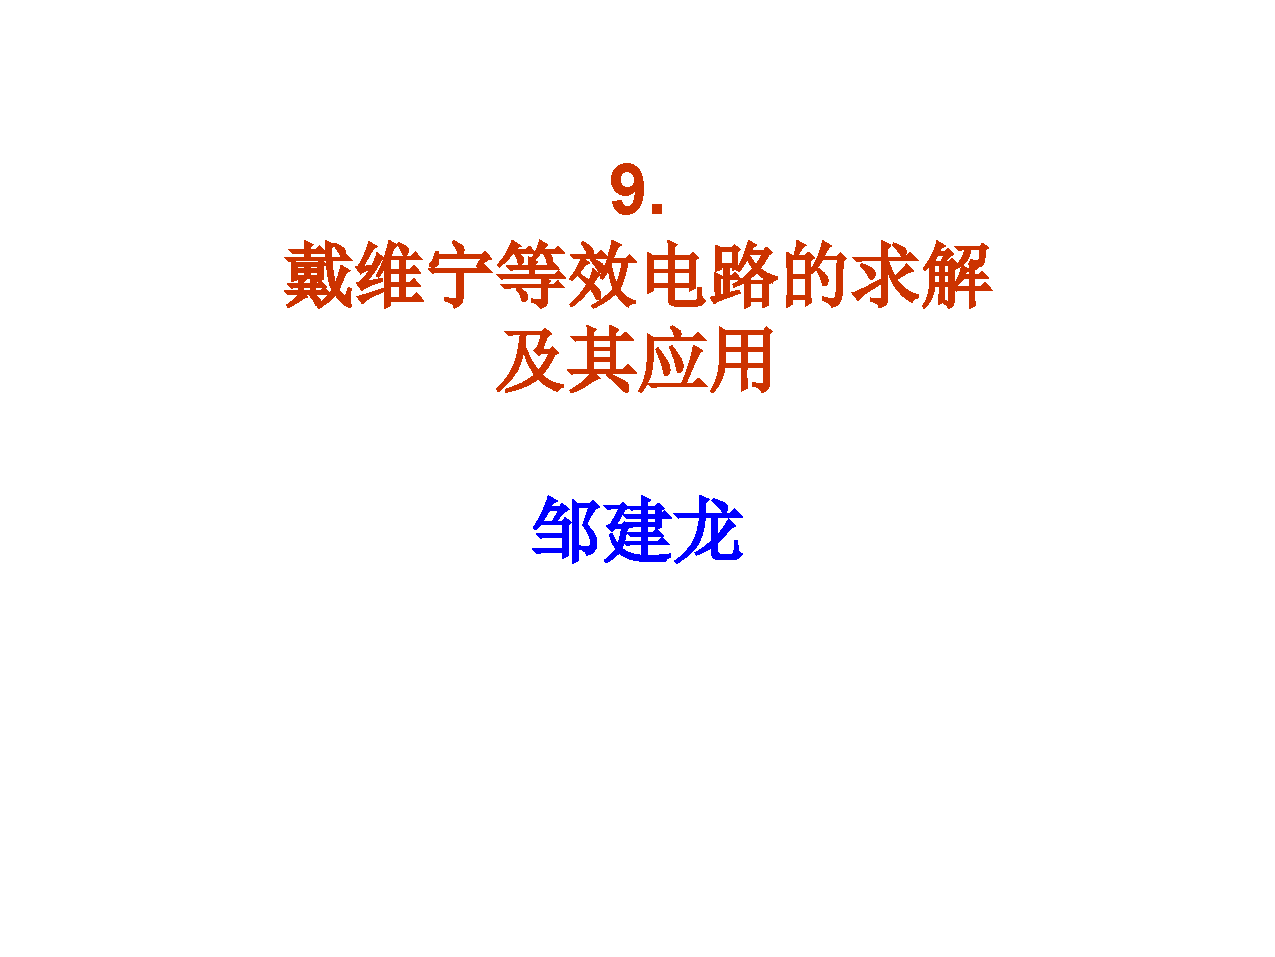
\includepdf[pages = - , nup=2x3]{content/Circuit(8).pdf}
\addcontentsline{toc}{chapter}{10 特勒根定理、互易定理和对偶原理}
\includepdf[pages = - , nup=2x3]{content/Circuit(9).pdf}
\addcontentsline{toc}{chapter}{11 电容、电感、动态电路的方程和初始条件}
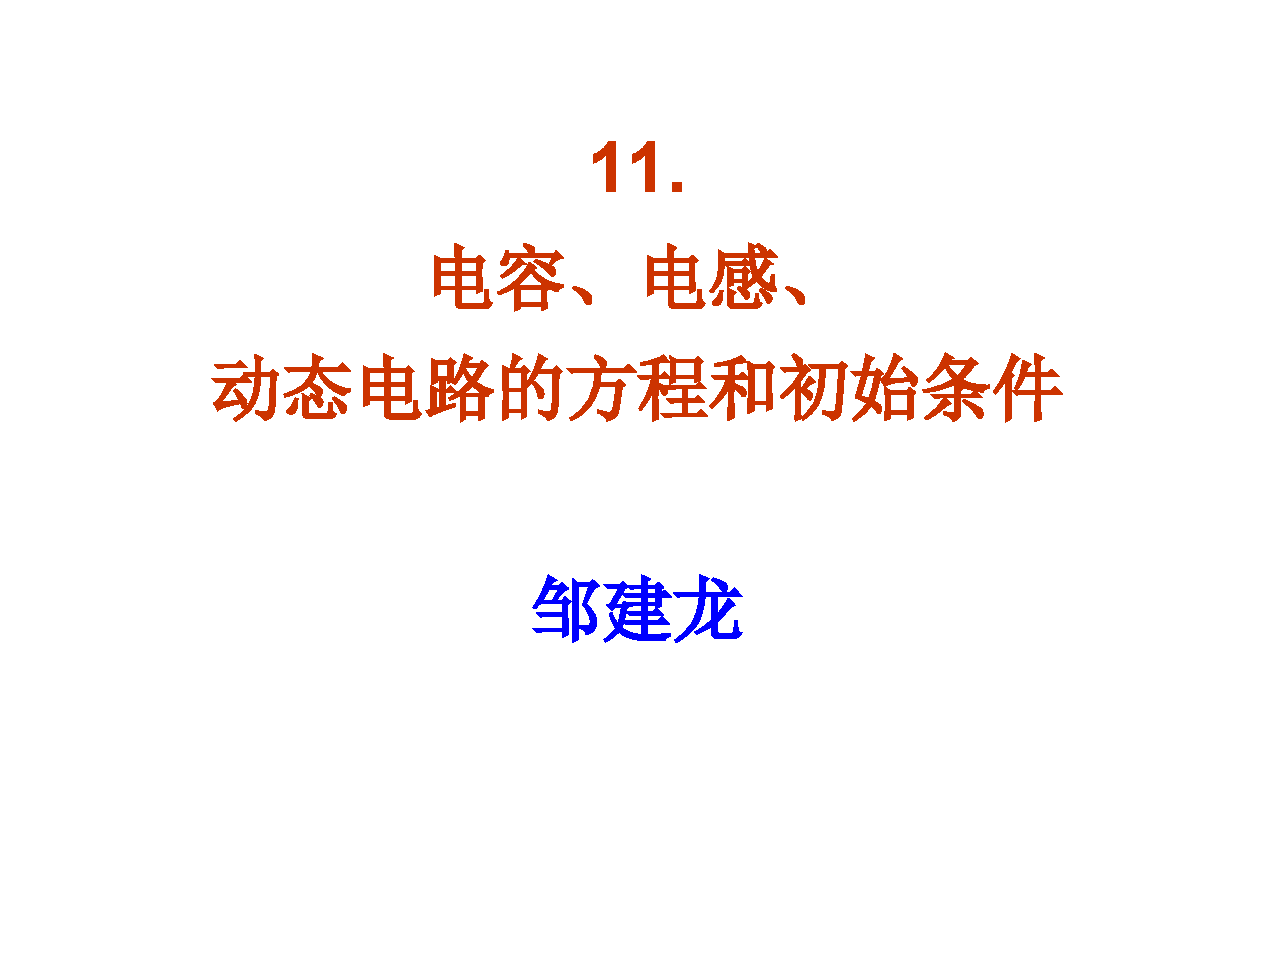
\includepdf[pages = - , nup=2x3]{content/Circuit(10).pdf}
\addcontentsline{toc}{chapter}{12 一阶电路的求解}
\includepdf[pages = - , nup=2x3]{content/Circuit(11).pdf}
\addcontentsline{toc}{chapter}{13 一阶电路的求解续}
\includepdf[pages = - , nup=2x3]{content/Circuit(12).pdf}
\addcontentsline{toc}{chapter}{14 二阶电路}
\includepdf[pages = - , nup=2x3]{content/Circuit(13).pdf}
\addcontentsline{toc}{chapter}{15 正弦稳态电路的相量法}
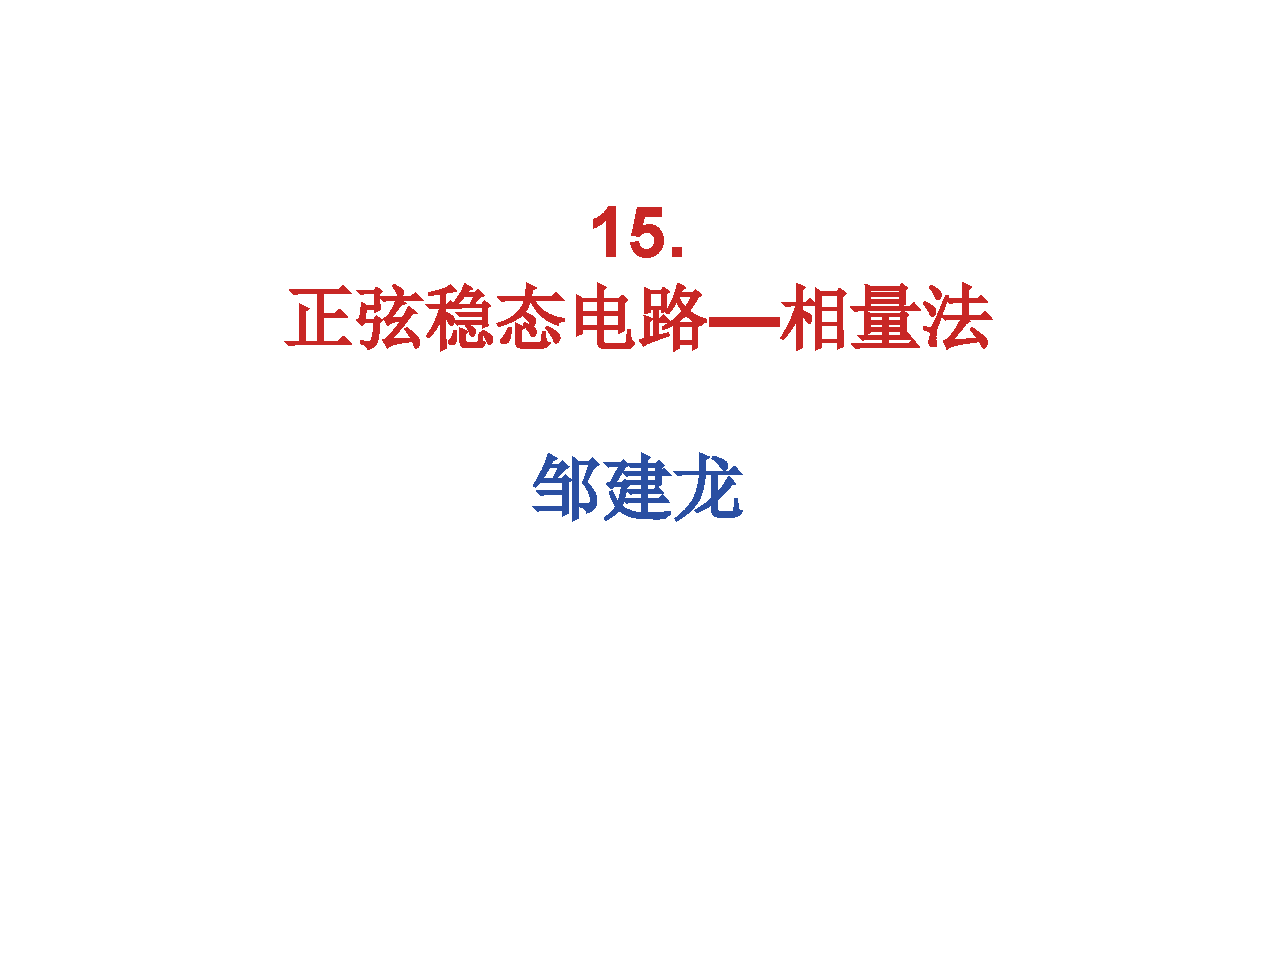
\includepdf[pages = - , nup=2x3]{content/Circuit(14).pdf}
\addcontentsline{toc}{chapter}{16 正弦稳态电路的求解}
\includepdf[pages = - , nup=2x3]{content/Circuit(15).pdf}
\addcontentsline{toc}{chapter}{17 正弦稳态电路的功率}
\includepdf[pages = - , nup=2x3]{content/Circuit(16).pdf}
\addcontentsline{toc}{chapter}{18 互感}
\includepdf[pages = - , nup=2x3]{content/Circuit(17).pdf}
\addcontentsline{toc}{chapter}{19 变压器}
\includepdf[pages = - , nup=2x3]{content/Circuit(18).pdf}
\addcontentsline{toc}{chapter}{20 对称和不对称三相电路}
\includepdf[pages = - , nup=2x3]{content/Circuit(19).pdf}
\addcontentsline{toc}{chapter}{21 三相电路的功率}
\includepdf[pages = - , nup=2x3]{content/Circuit(20).pdf}
\addcontentsline{toc}{chapter}{22 网络函数、滤波器}
\includepdf[pages = - , nup=2x3]{content/Circuit(21).pdf}
\addcontentsline{toc}{chapter}{23 谐振}
\includepdf[pages = - , nup=2x3]{content/Circuit(22).pdf}
\addcontentsline{toc}{chapter}{24 非正弦周期电路}
\includepdf[pages = - , nup=2x3]{content/Circuit(23).pdf}
\addcontentsline{toc}{chapter}{25 二端口网络}
\includepdf[pages = - , nup=2x3]{content/Circuit(24).pdf}
\addcontentsline{toc}{chapter}{26 运算放大器}
\includepdf[pages = - , nup=2x3]{content/Circuit(25).pdf}

\end{document}